In this section, we overview the existing approaches to Knowledge Base Question Answering (KBQA), as our approach, described in the next section, builds upon and extends some of these efforts. 

Recently, KBQA systems have converged to two major approaches: {\em semantic parsing}, and {\em information extraction} (IE) \cite{yao2014freebase}.
The former focuses on question understanding, and attempts to parse the sentences into a semantic representation, \eg logical forms \cite{Berant:EMNLP13,berant2014semantic,berant2015imitation}. The latter, information extracting approaches \cite{ACCU:2015,yih2015semantic,yao2014information} are based on identifying \textit{topical entities} in the question, and then, using pre-defined templates for mapping the question to predicates, explore the neighborhood of these entities in a KB.
Theoretically, semantic parsing-based systems would be capable of generating any required queries, and would apply to any question, seen or unseen in training, whereas the template-based approach is less likely to generalize. In practice, however, answers to most of the questions lie within two edge traversals within a KB, making the template (``information extraction''-based) approaches more effective.

Interestingly, one of the reasons for recent resurgence of interest in KBQA can be credited to creation of the WebQuestions dataset \cite{Berant:EMNLP13}, which is large enough to allow both comprehensive evaluation, and training machine learning methods. Thus, the performance of KBQA systems has quickly improved, with the current state of the art systems using the information extraction approach, with sophisticated ranking and matching postprocessing \cite{yih2015semantic}. Therefore, we chose to extend an existing KBQA system: Aqqu \cite{ACCU:2015}.
It follows an information extraction approach to KBQA and achieves one of the highest scores among publicly available systems.
However, as we will show, our approach is general and can be incorporated into other IE-based systems as well.


%One of the most popular benchmark datasets for knowledge base question answering is WebQuestions \cite{Berant:EMNLP13}, which has attracted a lot of attention recently and as a result the performance increased from 0.357 \cite{Berant:EMNLP13} to 0.525 \cite{yih2015semantic} in average F1 over test questions.
%The dataset is based on Freebase, which has been recently shut down\footnote{https://goo.gl/SZC3tg}.
%The shutdown of Freebase means that it will no longer be extended, but all the data will be available and it will be merged with WikiData\footnote{https://www.wikidata.org/}.
%Therefore, future datasets should probably use different reference KB, but there is no problem in using Freebase for experiments on existing benchmarks, such as WebQuestions.
%We should also stress, that the proposed approach isn't tied to Freebase and can be applied for question answering over dbPedia, WikiData or other knowledge bases.

%The focus of this work is on the fusion between structured data in the KB and unstructured text data.
%Therefore, we chose to extend an existing KBQA system: Aqqu \cite{ACCU:2015}.
%It follows an information extraction approach to KBQA and achieves one of the highest scores among publicly available systems.
%However, our approach can be incorporated into other systems as well.

We will first describe an information extraction approach to KBQA in more detail using Aqqu - our baseline system - as an example. Next, Section \ref{section:method} will present our system Text2KB, which extends this approach by incorporating external text-based data on various stages of the question answering process.

\begin{figure*}[!ht]
\centering
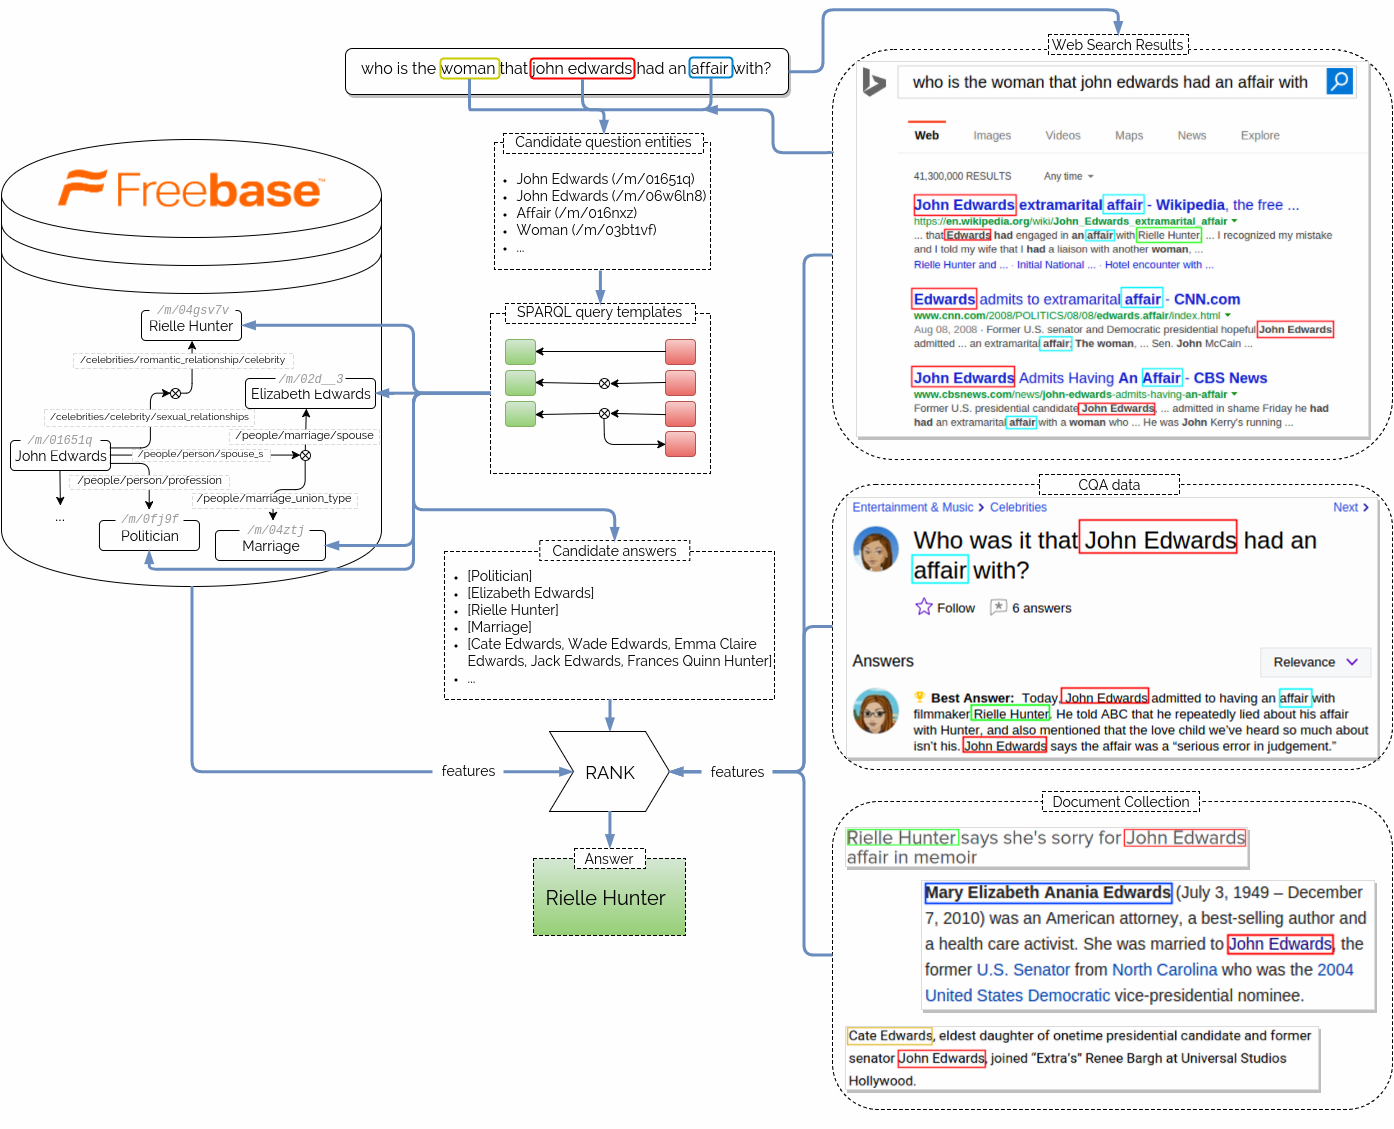
\includegraphics[width=0.9\textwidth]{img/Text2KB_model}
\vspace{-0.5cm}
\caption{The architecture of our Text2KB Question Answering system}
\label{fig:model}
\vspace{-0.5cm}
\end{figure*}


\subsection{The Aqqu KBQA system}
Recall, that a KBQA system first needs to identify question entities, which are used to initialize the ``neighborhood'' of potential answer entities in the KB that are connected to the question entities. For concreteness, consider a question from the Webquestions dataset \textit{``who is the woman that john edwards had an affair with?''}.
First, the system identifies a set of possible question entities.
In our example, entity \texttt{John Edwards} with Freebase mid \texttt{/m/01651q} is the main question entity.
However, Freebase contains millions of entities and it's often hard to identify the topical ones (\eg entities \texttt{Woman} and \texttt{Affair} are also present in Freebase) or to disambiguate and choose between \texttt{John Edwards} a politician (\texttt{/m/01641q}), \texttt{John Edwards} an American sports car racing driver (\texttt{/m/06zs089}) and other people with the same name.
There is even an entity with the name ``\texttt{had an affair with}''\footnote{http://www.freebase.com/m/0c0n01x}.
Aqqu considers all spans of terms under certain conditions on POS tags and use a dictionary of names, aliases and anchor texts \cite{SPITKOVSKY12.266} to map phrases to potential entities.
Most recent systems, including Aqqu, don't disambiguate entities at this stage and keep a set of candidates along with some information about their popularities and mention scores.

On the next stage, SPARQL query candidates are generated by exploring the neighborhood of the question topical entities usign a predefined set of query templates.
Each query template has an entity, predicate and answer entity placeholders.
Majority of the answers in WebQuestions dataset can be covered by just 3 templates (q\_entity - question entity, a\_entity - answer entity, cvt\_node - Freebase mediator node, which represent tuples with more than 2 arguments):

\begin{lstlisting}[frame=single,basicstyle=\small]
SELECT DISTINCT ?a_entity {
   <q_entity> <predicate> ?a_entity .
}
\end{lstlisting}

\vspace{-0.25cm}
\begin{lstlisting}[frame=single,basicstyle=\small]
SELECT DISTINCT ?a_entity {
   <q_entity> <predicate_1> ?cvt_node .
   ?cvt_node <predicate_2> ?a_entity .
}
\end{lstlisting}

\vspace{-0.25cm}
\begin{lstlisting}[frame=single,basicstyle=\small]
SELECT DISTINCT ?a_entity {
   <q_entity_1> <predicate_1> ?cvt_node .
   ?cvt_node <predicate_2> <q_entity_2> .
   ?cvt_node <predicate_3> ?a_entity .
}
\end{lstlisting}

The first template retrieves a set of entities that are directly connected to the given question entity via a certain predicate.
The second template accounts for the presence of a mediator node, that groups together arguments of a multi-argument relation.
And the last template looks for cases, when multi-argument relations also mention another question entity, \eg \texttt{Captain Kirk} and \texttt{Star Trek} for the question \textit{``who played captain kirk in star trek movie?''}.

%\begin{enumerate}
%\item \texttt{$[$q\_entity$]$ $\rightarrow$ $[$predicate$]$ $\rightarrow$ $[$a\_entity$]$}
%\item \texttt{$[$q\_entity$]$ $\rightarrow$ $[$predicate$_1]$ $\rightarrow$ $[$cvt\_entity$]$\\
%$[$cvt\_entity$]$ $\rightarrow$ $[$predicate$_2]$ $\rightarrow$ $[$a\_entity$]$}
%\item \texttt{$[$qentity$_1]$ $\rightarrow$ $[$predicate$_1]$ $\rightarrow$ $[$cvt\_entity$]$\\
%$[$cvt\_entity$]$ $\rightarrow$ $[$predicate$_2]$ $\rightarrow$ $[$q\_entity$_2]$\\
%$[$cvt\_entity$]$ $\rightarrow$ $[$predicate$_3]$ $\rightarrow$ $[$a\_entity$]$}
%\end{enumerate}

Finally, each query candidate is represented with a set of features, that includes information about the popularity of question entities (mention frequency), entity linking scores, size of the answer list, entity and predicate token matches, predicate score based on question token n-grams, \etc
The full list of features can be found in the original paper \cite{ACCU:2015}.
The final stage of the question answering process is filtering and ranking, using a trained random forest model. This ranking model, like the components of the other stages, is trained offline on the training subset of WebQuestions dataset.

\subsection{Basic system extensions}
In order to work with a high-performing KBQA system, before embarking on our drastic changes described in the next section, we analyzed and improved a number of details in the original Aqqu system, as described here. The improved system will be used as a baseline in the experiments of Section 5. 
First, we noticed that since Aqqu does not use information about answer entity Freebase types, in many cases it returns an answer that is type incompatible with the question: \eg state instead of county \etc
Similarly to how relations are scored in Aqqu, we decided to train a model to return a score, measuring a compatibility of the answer entities, using their notable types and question uni- and bigrams as features.
A second extension introduced a new date range query template, which, based on the error analysis, was lacking in Aqqu, but could be helpful. This template helps to solve the cases like \textit{``what team did david beckham play for in 2011?''}, where we need to look at the ranges of dates to figure out in which range does the specified date falls.

\vspace{-0.1cm}
\begin{lstlisting}[frame=single,basicstyle=\small]
SELECT DISTINCT ?a_entity {
   <q_entity_1> <predicate_1> ?cvt_node .
   ?cvt_node <from_predicate> ?date_from .
   ?cvt_node <to_predicate> ?date_to .
   ?cvt_node <predicate_2> ?a_entity .
   FILTER ( <question_date> >= ?date_from AND
            <question_date> <= ?date_to )
}
\end{lstlisting}
\vspace{-0.3cm}


%We also experimented with an additional template, which filters out lists by the entity notable types.

